\section{Assembler \& HCS08}

\subsection{HCS08 CPU Registers}

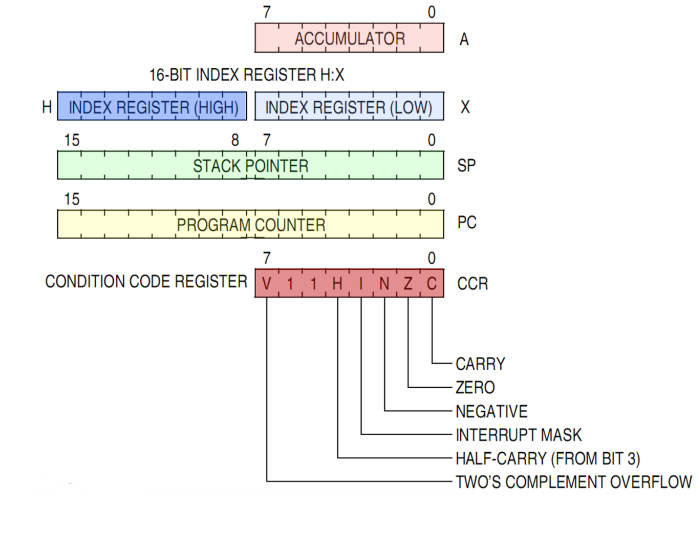
\includegraphics[width=0.5\textwidth]{hcs08-cpu-registers.png}

\textit{
    Registers the HCS08 contains:
}

\begin{itemize}
    \item{HX Register}
    \item{PC}
    \item{Akku}
    \item{Stack Pointer}
    \item{CCR}
\end{itemize}

\subsection{HCS08 Processor}

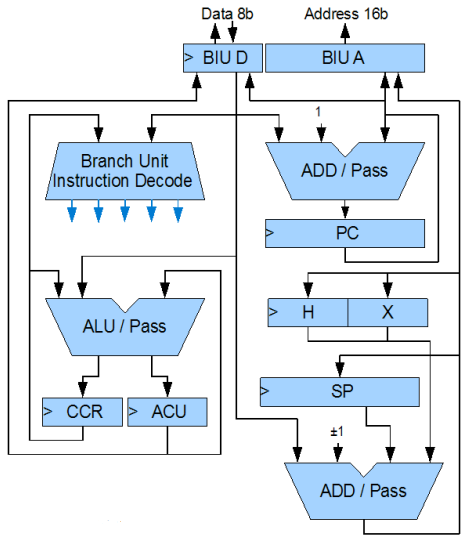
\includegraphics[width=0.5\textwidth]{hcs08-overview.png}

\begin{itemize}
    \item{8 Bit, Von Neumann archidecture}
    \item{\textbf{BIU} Bus Interface Unit}
    \item{\textbf{PC} Program Counter}
    \item{\textbf{ACU} Accumulator}
    \item{\textbf{ALU} Arithmetic Logic Unit}
    \item{\textbf{CCR} Condition Code Register (Collection of status flags)}
    \item{\textbf{SP} Stack (LI-FO, Pointer for Context and Parameter)}
    \item{\textbf{H:X} Index Register}
\end{itemize}

\subsection{Memory Mapping}

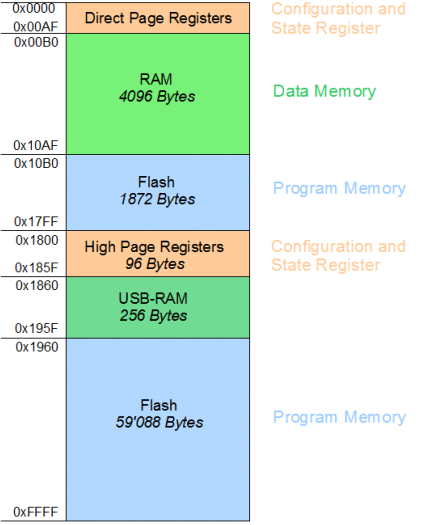
\includegraphics[width=0.5\textwidth]{hcs08-memory-mapping.png}

\textit{
    Access to the directpage (0x0000 - 0x0AF) needs less cycles,
    since the address is only 2 Bytes long.
}

\subsection{Register configuration HCS08}

\begin{lstlisting}
// define the dataflow direction input = 0 | output = 1
PTADD = 0x04;

// set output value
PTAD = 0x04;
// read value
uint_8 val = PTAD;

// set pullup enable port
PTADD = 0x00;
PTAPE = 0x04;
\end{lstlisting}

\begin{tabular}{rl}
    \textbf{Reg. Name} & \textbf{Description} \\
    PTxDD & \textit{Data Direction of Port x} \\
    PTxD  & \textit{Data value of Port x} \\
    PTxPE & \textit{Set Pullup Enable of Port x} \\
          & \textit{(PTxDD needs to be 0)} \\
\end{tabular}

\textit{
    \textbf{Pullup Enable} is used to pullup the value
    of the output to 1. This is usually used on a bus system
    to prevent a short circuit.
}

\subsection{Differences of Operations}

\textit{
    Comparing different operations, following should be taken
    in consideration:
}

\begin{itemize}
    \item{number of cycles}
    \item{memory usage, 8bit (directpage) / 16bit}
    \item{Set CCR bits / flags}
    \item{Used registers}
    \item{Address modes}
\end{itemize}
